%%%%%%%%%%%%%%%%%%%%%%%%%%%%%%%%%%%%%%%%%
% University/School Laboratory Report
% LaTeX Template
% Version 3.1 (25/3/14)
%
% This template has been downloaded from:
% http://www.LaTeXTemplates.com
%
% Original author:
% Linux and Unix Users Group at Virginia Tech Wiki 
% (https://vtluug.org/wiki/Example_LaTeX_chem_lab_report)
%
% License:
% CC BY-NC-SA 3.0 (http://creativecommons.org/licenses/by-nc-sa/3.0/)
%
%%%%%%%%%%%%%%%%%%%%%%%%%%%%%%%%%%%%%%%%%

%----------------------------------------------------------------------------------------
%	PACKAGES AND DOCUMENT CONFIGURATIONS
%----------------------------------------------------------------------------------------

\documentclass{article}

\usepackage{graphicx} % Required for the inclusion of images
\usepackage{amsmath} % Required for some math elements
\usepackage{enumitem}
\usepackage[section]{placeins}
\usepackage{gensymb}

\setlength\parindent{0pt} % Removes all indentation from paragraphs

\renewcommand{\labelenumi}{\alph{enumi}.} % Make numbering in the enumerate environment by letter rather than number (e.g. section 6)

\newlist{inlinelist}{enumerate*}{1}
\setlist*[inlinelist,1]{%
  label=(\arabic*),
}

%----------------------------------------------------------------------------------------
%	DOCUMENT INFORMATION
%----------------------------------------------------------------------------------------

\title{\begin{LARGE}
	\textbf{EE 445L - Lab 9: Temperature Data Acquisition System}
\end{LARGE}} % Title

\author{Joshua Bryant \\ jmb6357 \and James Morris \\ jsm3288} % Author name

\date{\today} % Date for the report

\begin{document}

\maketitle % Insert the title, author and date

%----------------------------------------------------------------------------------------
%	SECTION 1 Objectives
%----------------------------------------------------------------------------------------
\section{Objective}
	The goals of this lab are to study ADC conversion, the Nyquist Theorem, the Valvano Postulate, and their implications in real world analog systems. These concepts will be studies by developing a temperature measurement system using a thermistor.
%----------------------------------------------------------------------------------------
%	SECTION 2 Hardware Design
%----------------------------------------------------------------------------------------
\section{Hardware Design}
	\begin{figure}[h]
		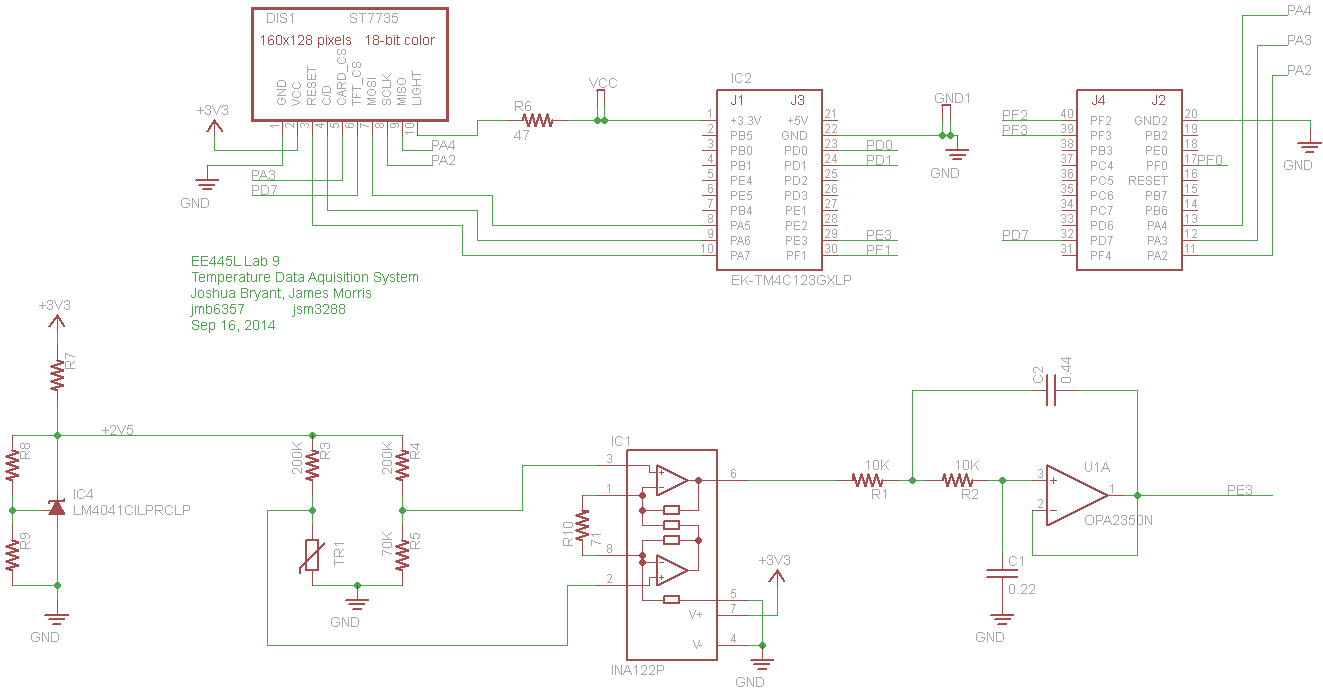
\includegraphics[keepaspectratio, width = 0.9\textwidth]{Lab9Graphics/circuit.png}
		\caption{Circuit diagram of the thermistor interface.}
	\end{figure}
%----------------------------------------------------------------------------------------
%	SECTION 3 Software Design
%----------------------------------------------------------------------------------------
%\section{Software Design}
%Not included in this report. It'll be submitted through canvas along with this PDF

%----------------------------------------------------------------------------------------
%	SECTION 4 Measurement Data
%----------------------------------------------------------------------------------------
\section{Measurement Data}
	\begin{enumerate}
		\item[1)] %Static Circuit Performance Measurements (Procedure 2
			\textbf{Static Circuit Performance Measurements: }\\
			\begin{table}[h]
				\centering			
				\begin{tabular}{|c|c|c|c|}\hline
					Resistance ($\Omega$) & Themistor Circuit Output (V) & LPF Output (V) & ADC Value \\ \hline
					Open ($\infty$)	&	3.32	&	0.334	&	4025	\\ \hline
					110K 			&	2.84	&	0.282	&	3375	\\ \hline
					100K			&	2.52	&	0.254	&	3046	\\ \hline
					92K				&	2.36	&	0.234	&	2790	\\ \hline
					82K				&	2.04	&	0.202	&	2420	\\ \hline
					72K				&	1.72	&	0.166	&	1965	\\ \hline
					62k				&	1.32	&	0.130	& 	1525	\\ \hline
					Short (0$\Omega$)&	0.12	&	0.01	&	5		\\ \hline			
				\end{tabular}
			\end{table}
			
		\item[2)] %Dynamic Circuit Performance (Procedure 3)
			\textbf{Dynamic Circuit Performance: }\\
			\begin{table}[h]
				\centering
				\begin{tabular}{|c|c|c|c|}\hline
					Frequency (Hz)	&	Input (V)	&	Output (V)	&	Gain (Vout/Vin)\\ \hline
					1	&	0.008	&	0.160	&	20\\ \hline
					2	&	0.008	&	0.160	&	20\\ \hline
					3	&	0.008	&	0.240	&	30\\ \hline
					4	&	0.008	&	0.140	&	17.5\\ \hline
					5	&	0.008	&	0.120	&	15\\ \hline
					6	&	0.008	&	0.170	&	21.25\\ \hline
					7	&	0.008	&	0.200	&	25\\ \hline
					8	&	0.008	&	0.216	&	27\\ \hline
					9	&	0.008	&	0.232	&	29\\ \hline
					10	&	0.008	&	0.240	&	30\\ \hline
					15	&	0.008	&	0.248	&	31\\ \hline
					20	&	0.008	&	0.240	&	30\\ \hline
					25	&	0.008	&	0.224	&	28\\ \hline
					30	&	0.008	&	0.216	&	27\\ \hline
					35	&	0.008	&	0.224	&	28\\ \hline
					40	&	0.008	&	0.224	&	28\\ \hline
				
				\end{tabular}
			\end{table}
			
			\begin{figure}[h]
				\centering
				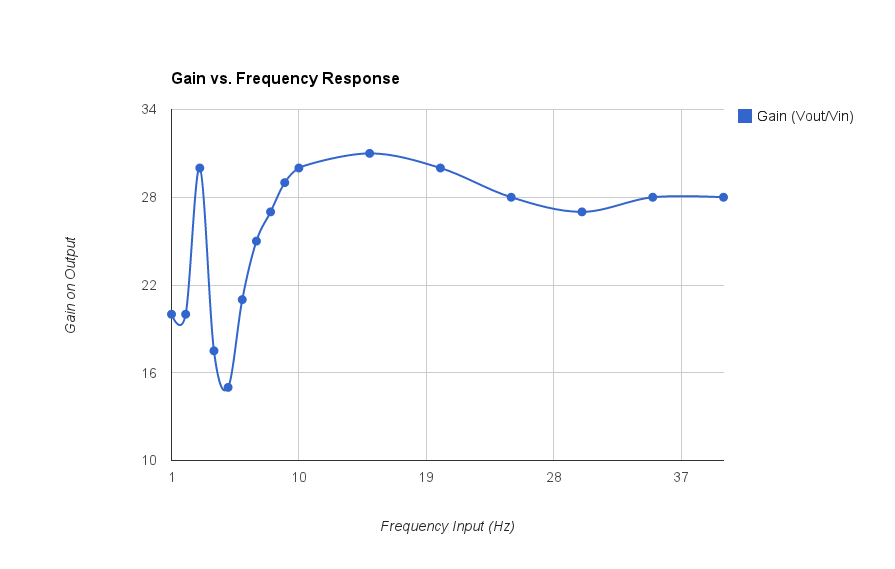
\includegraphics[keepaspectratio, width = \textwidth]{Lab9Graphics/GainFrequencyResponse.png}
				\caption{Gain Frequency response of our thermistor interface circuit and the low pass filter from the data above.}
			\end{figure}
			\pagebreak
			
		\item[3)] %Accuracy (Procedure 6)
			\textbf{Accuracy: }\\[-2.5ex]
			\begin{table}[h]
				\centering
				\begin{tabular}{|c|c|}\hline
					Fluke Value (\celsius)	&	Thermistor Circuit Value (\celsius)\\ \hline
					33	&	33.62\\ \hline
					33	&	33.20\\ \hline
					33	&	33.35\\ \hline
					33	&	33.54\\ \hline
					33	&	33.23\\ \hline
				\end{tabular}
			\end{table} \\[-1ex]
			The average accuracy for the thermistor circuit is 0.388\celsius.
			%\pagebreak
			
		\item[4)]
			\textbf{Reproducibility}\\[-1ex] %Reproducibility (Procedure 7)
			\begin{table}[h]
				\centering
				\begin{tabular}{|c|c|}\hline
					Measurement Number	&	Thermistor Circuit Value (\celsius)\\ \hline
					1	&	29.27\\ \hline
					2	&	29.41\\ \hline
					3	&	29.43\\ \hline
					4	&	29.36\\ \hline
					5	&	29.40\\ \hline
					6	&	29.44\\ \hline
					7	&	29.45\\ \hline
					8	&	29.42\\ \hline
					9	&	29.53\\ \hline
					10	&	29.63\\ \hline
				\end{tabular}
			\end{table} \\[-1ex]
			The standard deviation for our system was 0.096\celsius.
	\end{enumerate}
%----------------------------------------------------------------------------------------
%	SECTION 5 Analysis and Discussion
%----------------------------------------------------------------------------------------
\section{Analysis and Discussion}
	\begin{enumerate}
		\item% What is the Nyquist theorem and how does it apply to this lab?
			The Nyquist Theorem is the theorem that states an signal must be sampled at a frequency at least twice it's largest frequency component in order to be sampled correctly. It applies to this lab because we must know the maximum frequency we wish to sample in order to design the low pass filter to cut out most signals above twice this frequency so we get better results from our ADC and reduce the error in the system.
		\item% Explain the difference between resolution and accuracy.
			Resolution is the smallest difference between values which your system is able to measure. Accuracy is how closely the output value of the system matches what it is actually measuring.
		\item% What is the purpose of the LPF?
			The low pass filter is supposed to remove all frequencies above twice the frequency at which we are sampling to reduce aliasing. The reason this works is the low pass filter is being implemented in hardware meaning the signal is not being digitized before sampling. This reduces the aliasing encountered and reduces the computational load on the micro controller considerably.
		\item% If the R versus T curve of the thermistor is so nonlinear, why does the voltage versus temperature curve look so linear?
			The values of the components chosen for the thermistor circuit and the gain of the instrumentation amplifier helped to "spread out" the exponential decay and make it to where it can be approximated as multiple short linear segments along the curve.
		\item% There are four methods (a,b,c,d) listed in the 4) Software Conversion section of methods and constraints. For one of the methods you did not implement, give reasons why your method is better, and give reasons why this alternative method would have been better.
			One method we did not choose was to implement a large table lookup. The reason was due to memory constraints on the side of our compiler since it would not support flashing that much memory on the board. We implemented a small table lookup with linear interpolation in between data points to reduce the amount of memory that was needed. However, our method requires more computational time than looking up the ADC value and results in slightly more error in the output value due to a linear interpolation of a non-linear signal.
	\end{enumerate}

\end{document}